\section{Методы кластеризации пользователей}

\subsection{Постановка задачи}

Рассмотрим задачу кластеризации пользователей социальных сетей для целевой рекламы с использованием нейронных сетей. На вход алгоритма кластеризации подается индентификатор пользователя социальной сети. Выходом алгоритма является номер кластера, или же индекс целевой рекламы, которая интересна пользователю. Таким образом, задача персонализации пользователя делится на 2 этапа: получения доступной информации о пользователе из социальной сети и определение к какому кластеру пользователь относится. Постановка задачи представлена на рисунке \ref{fig:a0}.

\begin{figure}[hbtp]
	\centering
	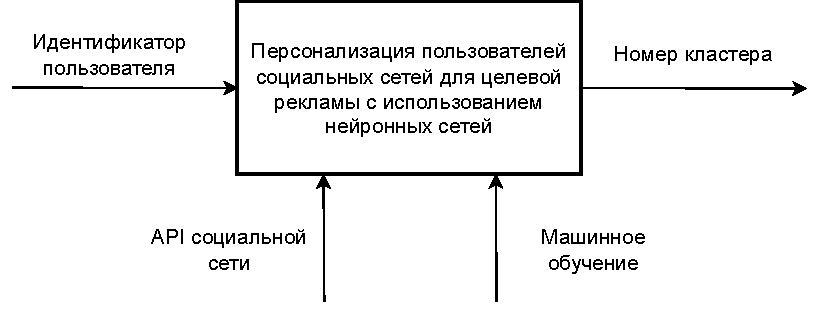
\includegraphics[scale=0.8]{img/a0.pdf}
	\caption{Постановка задачи}
	\label{fig:a0}
\end{figure}

\subsection{Обзор существующих решений}

Сегодня существует множество хороших решений для рекомендательных систем для многих бизнес-областей. У большинства социальных сетей есть собственные алгоритмы персонализации пользователей для предоставления рекламы различных товаров или услуг. 

\subsubsection{Facebook}
У Facebook самая сложная модель ранжирования. Она учитывает множество различных факторов. Техническая реализация находится в закрытом доступе. Решение состоит из алгоритмов и методов, каждый из которых позволяет учитывать конкретный атрибут или явление в среде, решать определенную проблему. Facebook развивает систему итеративно и регулярно публикует обновление списка атрибутов, влияющих на ранжирование и основные принципы. Итеративность и постоянное развитие — неотъемлемые элементы хорошей рекомендательной системы.

\subsubsection{ВКонтакте}
Социальная сеть ВКонтакте использует сервис под названием <<Церебро Таргет>> для мониторинга открытых действий своих пользователей, сбора и систематизации полученных данных. Этот сервис используется для получения портрета необходимой целевой аудитории и определения места ее сосредоточения. Данный сервис является платным.

\subsubsection{Yandex Zen}
Дзен лента – это интеллектуальная алгоритмическая программа, которая анализирует публикуемый писателем материал и рекомендует его читателям в соответствии с их интересами. Таким образом информация распространяется по определенным направлениям. 

Яндекс.Дзен способен предоставлять пользователям персонализированный контент.  Платформа использует алгоритмы машинного обучения, чтобы рекомендовать новости пользователям на основе их предыдущего взаимодействий с площадкой или поисковой системой. Данные алгоритмы находятся в закрытом доступе.

\subsection{Выбор социальной сети для получения информации о пользователях}
Для формирования обучающей выборки необходимо выбрать наиболее подходящую социальную сеть, в которой зарегистрировано множество пользователей, а также такую, которая предоставляет данные о своих пользователях в открытом доступе.

\subsubsection{Социальная сеть ВКонтакте}
Социальной сетью ВКонтакте пользуется более 50 млн человек в день. Она является крупнейшей социальной сетью в России и странах СНГ. Основным преимуществом данной сети является открытое и бесплатное API, которое позволяет собирать большое количество информации о пользователях социальных сетей. Также аудитория ВКонтакте является в большей части русскоязычной.

\subsubsection{Социальная сеть Facebook}
Социальная сеть Facebook появилась в 2004 году как внутренняя социальная сеть в Гарвардском университете. Несмотря на то, что он начинал как способ поддержания связи, он стал удобным инструментом бизнеса, который мог точно нацеливаться на аудиторию и доставлять рекламу людям, которые, скорее всего, захотят их продукты или услуги.

По данным компании, ежедневно в Facebook заходят 1,28 млрд человек.

Также Facebook имеет открытое API для доступа к большому количеству информации.

Основной проблемой является то, что 4 марта 2022 году было принято решение о блокировке доступа к сети на территории Российской Федерации.

\subsubsection{Социальная сеть Twitter}
Twitter - американский сервис блогов и социальная сеть, в которой пользователи публикуют сообщения и взаимодействуют с ними. Пользователи взаимодействуют с «Твиттером» через браузер, мобильное приложение или через API.

Проблемой данной социальной сети является то, что нельзя собрать много информации о пользователях, а также с 4 марта 2022 года социальная сеть Twitter заблокирована на территории Российской Федерации.

\subsubsection{Вывод}
В качестве выбранной социальной сети для получения информации о людях была выбрана сеть ВКонтакте, так как у нее есть открытое API, большое количество информации о пользователях, а самое главное -- она доступна на территории Российской Федерации.

\subsection{Алгоритмы решения задач кластеризации}
Кластеризация (или кластерный анализ) \cite{ershov2016} -- это задача разбиения множества объектов на группы, называемые кластерами.

Главное отличие кластеризации от классификации состоит в том, что перечень групп четко не задан и определяется в процессе работы алгоритма. 

\subsubsection{K-means++}

Алгоритм k-средних является наиболее известным и используемым методом кластеризации. 

Кластеризация k-means широко изучалась с различными расширениями в литературе и применялась в различных существенных областях \cite{alhawarat2018revisiting}.

Данный метод разбивает множество элементов векторного пространства на заранее известное число кластеров. Алгоритм стремится минимизировать среднеквадратичное отклонение на точках каждого кластера. 

Основная идея данного алгоритма заключается в том, что на каждой итерации заново вычисляется центр масс для каждого кластера, полученного на последнем шаге, затем векторы разбиваются на кластеры вновь в соответствии с тем, какой из новых центров оказался ближе по выбранной метрике. Алгоритм завершается, когда на какой-то итерации не происходит изменения кластеров.

Интуитивно алгоритм инициализации использует тот факт, что хорошая кластеризация относительно распределена, поэтому при выборе нового центра кластера предпочтение следует отдавать тем, которые находятся дальше от ранее выбранных центров.

Основная идея модифицированного K-means++ состоит в том, чтобы выбирать центры один за другим контролируемым образом, где текущий набор выбранных центров будет стохастически смещать выбор следующего центра \cite{bahmani2012scalable}.

Вычисление цетроида:
\begin{equation}
	\text{centroid}(Y) = \frac{1}{|Y|} \sum_{y \in Y} y
\end{equation}

Необходимо определить стоимость $Y$ по отношению к $C$ как:
\begin{equation}
	\phi_Y(C) = \sum_{y \in Y} d^2 (y, C) = \sum_{y \in Y} \text{min}_{i=1..k} ||y-c_i||^2
\end{equation}

Целью кластеризации k-средних является выбор набора $C$ из $k$ центров для минимизации $\phi_X(C)$.

Основным недостатком инициализации k-means++ с точки зрения масштабируемости является присущий ей последовательный характер: выбор следующего центра зависит от текущего набора центров. Также необходимо знать изначальное количество кластеров.

\subsubsection{Нейронные сети}
Нейронные сети позволяют быстро, а также эффективно решать задачи кластеризации. Основное преимущество нейронных сетей заключается в том, что они хорошо приспособлены для параллельных вычислений и обучаемые.

Качество нейронной сети зависит от данных, на которых она обучается, и от того, насколько верно подобрали ее структуру. Предобработка данных \cite{claster_neural} -- это преобразование статистического набора данных.

На входы нейронной сети подаются значения признаков выбранного объекта. Нейросеть обрабатывает эти сигналы, после чего в выходном слое определяется нейрон-победитель. Нейрон-победитель выходного слоя определяет класс объекта, признаки которого были поданы на входы нейросети.

Такой подход к кластеризации особенно необходим при работе с большими объемами данных, требующими больших затрат вычислительной мощности и машинного времени.

Преимущества данного метода:
\begin{enumerate}
	\item[1)] устойчивость к шумам входных данных;
	\item[2)] адаптация к изменениям;
	\item[3)] отказоустойчивость;
	\item[4)] быстродействие.
\end{enumerate}

Недостатки:
\begin{enumerate}
	\item[1)] неточность ответа
	\item[2)] принятие решений в несколько этапов;
	\item[3)] вычислительные задачи.
\end{enumerate}

\subsubsection{Fuzzy C-means}
Существует множество методов нечеткой кластеризации. Среди них широко используется алгоритм нечетких C-средних (FCM). Он основан на концепции нечеткого C-разбиения. Данный алгоритм и его производные очень успешно использовались во многих приложениях, таких как распознавание образов, классификация, интеллектуальный анализ данных и сегментация изображений.

Обычно алгоритм С-means состоит из нескольких этапов выполнения. На первом шаге алгоритм случайным образом выбирает C начальных центров кластера из исходного набора данных. Затем, на более поздних этапах, после некоторых итераций алгоритма, конечный результат сходится к фактическому центру кластера. Поэтому выбор хорошего набора начальных центров кластера очень важен для алгоритма FCM. Однако трудно случайным образом выбрать хороший набор начальных кластерных центров. Если выбран хороший набор начальных центров кластера, алгоритму может потребоваться меньше итераций, чтобы найти фактические центры кластера.

Нечеткий алгоритм c-means минимизирует величину 
\begin{equation}
	\sum_{i=1}^{|X|} \sum_{j=1}^C u_{i,j}^m ||x_i - c_j||^2, 1 \leq m \leq \infty,
\end{equation}
ге $m \in R$, $u_{i,j}$ - коэффициент принадлежности вектора $x_i$ к кластеру $c_j$, $x_i$ - i-ый компонент $|X|$-мерного вектора $X$, $C$ - количество кластеров, $c_j$ - центр j-го кластера, а $|| * ||$ - норма, которая определяет расстояние от вектора до центра кластера.

Преимуществом данного алгоритма является то, что он является нечетким и каждый из объектов принадлежит всем кластерам с разной степенью принадлежности.

Недостатками является то, что из-за того, что данный алгоритм является нечетким, он требует больших вычислительных затрат. Также необходимо заранее знать количество кластеров. Алгоритм очень чувствителен к выбору начальных центров кластеров.

\subsubsection{Гауссовы смеси} 
Существует категория методов кластеризации, которые определяют кластеры как наблюдения, имеющие, скорее всего, одинаковое распределение \cite{maugis2013adaptive}. В этом последнем случае предполагается, что каждая субпопуляция распределена по параметрической плотности, подобной гауссовой, и, таким образом, неизвестная плотность данных представляет собой смесь этих распределений.

На практике каждый кластер представлен параметрическим распределением, подобным гауссову, и весь набор данных моделируется смесью этих распределений \cite{schieferdecker2009gaussian}. Преимущество кластеризации на основе моделей заключается в обеспечении строгой структуры для оценки количества кластеров и роли каждой переменной в процессе кластеризации

Чем больше информации у нас есть о каждом человеке, тем лучше ожидается, что метод кластеризации будет работать. Однако структура, представляющая интерес, часто может содержаться в подмножестве доступных переменных, и многие переменные могут быть бесполезными или даже вредными для обнаружения разумной структуры кластеризации. Таким образом, важно выбрать соответствующие переменные с точки зрения кластерного анализа.

Распределение Гаусса, также называемое нормальным распределением, представляет собой непрерывное распределение вероятностей:
\begin{equation}
	N(X|\mu, \Sigma) = \frac{1}{(2\pi)^{\frac{D}{2}} \sqrt{|\Sigma|}} \exp{-\frac{(X-\mu)^T\Sigma^{-1}(X-\mu)}{2}},
\end{equation}
где $\mu$ - D-мерный средний вектор, $\Sigma$ - D x D ковариационная матрица, которая описывает форму Гаусса и $|\Sigma|$ обозначает определитель $\Sigma$.

Модель Гауссовых смесей представляется в виде линейной комбинации базового распределения веротностей по Гауссу и выражается как
\begin{equation}
	p(X) = \sum_{k=1}^{K}\pi_kN(X|\mu_k, \Sigma_K)
\end{equation}

\subsubsection{Вывод}
Возможность обучения является одним из главных преимуществ нейронных сетей перед остальными методами. В процессе обучения нейронная сеть способна выявлять сложные зависимости между входными данными и выходными, а также выполнять обобщение. Это значит, что в случае успешного обучения сеть сможет вернуть верный результат на основании данных, которые отсутствовали в обучающей выборке, а также неполных и/или «зашумленных», частично искажённых данных.

Также на вход нейронной сети можно передавать не предобработанные (сырые) данные. У других рассмотренных методов основным недостатком является неустойчивость к шумам.

\subsection{Классификация нейронных сетей для решения задачи кластеризации пользователей социальных сетей}

\subsubsection{Сети адаптивного резонанса}
Теория адаптивного резонанса (АРТ) имеет биологическую мотивацию и является крупным достижением в парадигме конкурентного обучения \cite{du2010clustering}. Теория приводит к серии неконтролируемых сетевых моделей в реальном времени для кластеризации, распознавания образов и ассоциативной памяти.

Модели способны к стабильному распознаванию категорий в ответ на произвольные входные последовательности с быстрым или медленным обучением. Модели ART характеризуются системами дифференциальных уравнений, которые формулируют устойчивые самоорганизующиеся методы обучения. 

На этапе обучения сохраненный прототип категории адаптируется, когда шаблон ввода достаточно похож на прототип. Когда обнаруживается новизна, ART адаптивно и автономно создает новую категорию с исходным шаблоном в качестве прототипа.

Основным модулем обработки любой сети ART является конкурентоспособная обучающая сеть. Нейроны $m$ входного слоя $F_1$ регистрируют значения входного шаблона $I = (i_1, i_2, ..., i_m)$. Каждый нейрон выходного слоя $F_2$ получает восходящую сетевую активность $t_j$, построенную из всех выходов $F_1$. Векторные элементы $T=(t_1,...,t_n)$ можно рассматривать как результаты сравнения между входным шаблоном $I$ и прототипами $W_1=(w_{11},...,w_{1m}),...,W_n=((w_{n1},...,w_{nm})$. Эти прототипы хранятся в синаптических весах соединений между $F_1$ и $F_2$-нейронами. Единственный $F_2$-нейрон $J$, получающий самую высокую чистую активность $t_J$, устанавливает свой выходной сигнал равным единице, в то время как все остальные выходные нейроны остаются равными нулю
\begin{equation}
	\begin{matrix}
		u_i & =
		& \left\{
		\begin{matrix}
			1 & \mbox{если } t_j > \text{max}(t_k : k \neq j) \\
			0 & \mbox{иначе. }
		\end{matrix} \right.
	\end{matrix}
\end{equation}

Одним из возможных способов вычисления чистой активности и с помощью этого измерения сходства между и является взвешенная сумма

\begin{equation}
	t_j = \sum_{i=1}^{m}w_{ij} i_i
\end{equation}

Часто используются вариации этого показателя, поскольку значение оказывает большое влияние на результирующие кластеры. После того, как $F_2$ победитель $J$ был найден, соответствующий прототип $W_J=(w_{iJ},...,w_{mJ})$ адаптируется к входному шаблону $I$. Одним из подходящих методов адаптации является небольшое смещение в сторону входного шаблона.

\begin{equation}
	W_J^{\text{new}}=\eta I + (1- \eta) W_J^{\text{old}}
\end{equation}

Недостатками данной сети является то, что она имеет большое количество синаптических связей в сети. При этом многие из обучающих весов после обучения оказываются нулевыми. Также результат часто зависит от порядка обучающей выборки.

\subsubsection{Сети Кохонена}
Сети (слои) Кохонена относятся к самоорганизующимся нейронным сетям \cite{gorba4enko2010seti}. Самоорганизующаяся сеть позволяет выявлять кластеры (группы) входных векторов, обладающих некоторыми общими свойствами. 

Кластеризация позволяет сгруппировать сходные данные, что облегчает решение ряда задач Data Mining: 
\begin{enumerate}
	\item[1)] изучение данных, облегчение анализа;
	\item[2)] прогнозирование;
	\item[3)] обнаружение аномалий.
\end{enumerate}

С помощью сетей Кохонена производится кластеризация объектов, описываемых количественными характеристиками. 

Сеть (слой) Кохонена (рисунок \ref{fig:kohonen}) — это однослойная сеть, построенная из
нейронов типа WTA (Winner Takes All — победитель получает все).

\begin{figure}[hbtp]
	\centering
	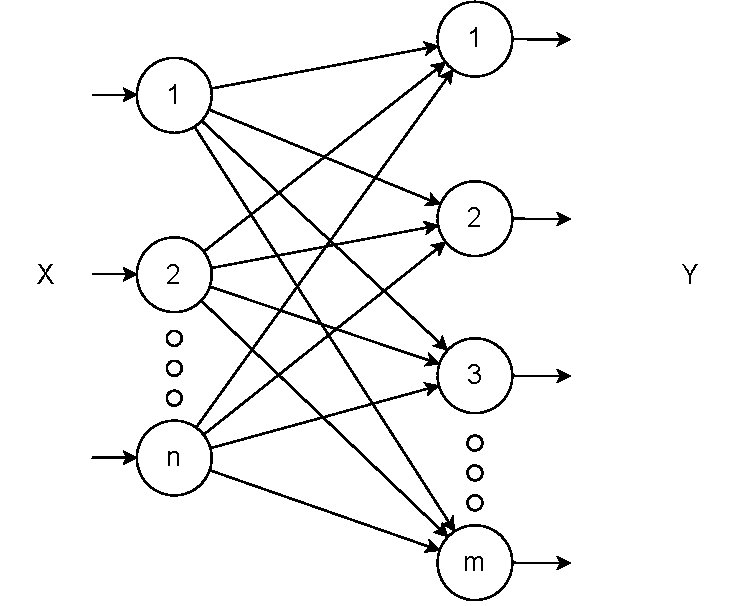
\includegraphics[scale=1]{img/koh.pdf}
	\caption{Структура сети Кохонена\cite{koh}}
	\label{fig:kohonen}
\end{figure}

Для обучения сети применяются механизмы конкуренции. Перед процессом обучения производится инициализация сети, то есть первоначальное задание векторов весов. В простейшем случае задаются случайные значения весов. Процесс обучения сети Кохонена состоит из циклического повторения ряда шагов: 
\begin{enumerate}
	\item[1)] подача исходных данных на входы;
	\item[2)] нахождение выхода каждого нейрона;
	\item[3)] определение <<выигравшего>> нейрона;
	\item[4)] корректировка весов <<выигравшего>> нейрона по правилу Кохонена;
	\item[5)] переход на шаг 1, если обучение не завершено.
\end{enumerate}

Алгоритм учитывает евклидово расстояние между двумя n-мерными векторами, которое измеряется сходством между входными векторами \cite{nizam2010kohonen}. Расстояние входного вектора от каждого нейрона i, $D_i$ задается формулой
\begin{equation}
	D_i = ||W_{ij} - X|| = \sqrt{\sum_{j=1}^{n}(x_j - w_{ij})^2}
\end{equation}
где $X = (x_1,...,x_n)^{\text{T}}$ обозначает входной вектор $w_{ij}=(w_{11},...,w_{im})^{\text{T}}$.

Победителем объявляется Кохонен с минимальной дистанцией. Другими словами, вектор веса победителя находится ближе всего к входному вектору.

\begin{equation}
	D_w = \text{min} \{D_i\}, i \in \{1,2,...,m\}
\end{equation}

Во время обучения победитель настраивает свои веса так, чтобы они были ближе к значениям данных, а соседи победителя также настраивают свои веса так, чтобы они были ближе к тому же вектору входных данных в соответствии со следующим соотношением

\begin{equation}
	W_i = W_{ij} + \alpha (W_i - X), i=\{1,2,...,m\}
\end{equation}

Таким образом, части сети конкурируют за выбор. Только веса победителя будут адаптированы. Настройка соседнего нейрона играет важную роль в сохранении порядка входных данных. Таким образом, выигравший нейрон находится ближе всего к входному значению. После обучения весовые векторы самоорганизуются и представляют собой прототипы классов входного вектора.

\subsubsection{Перцептрон без учителя}
В основе перцептрона лежит математическая модель восприятия информации мозгом. Разные исследователи по-разному его определяют. В самом общем своем виде (как его описывал Розенблатт) он представляет систему из элементов трех разных типов: сенсоров, ассоциативных элементов и реагирующих элементов.

Перцептрон стал одной из первых моделей нейросетей. На рисунке \ref{fig:Simple_perceptron} представлена схема перцептрона.

\begin{figure}[hbtp]
	\centering
	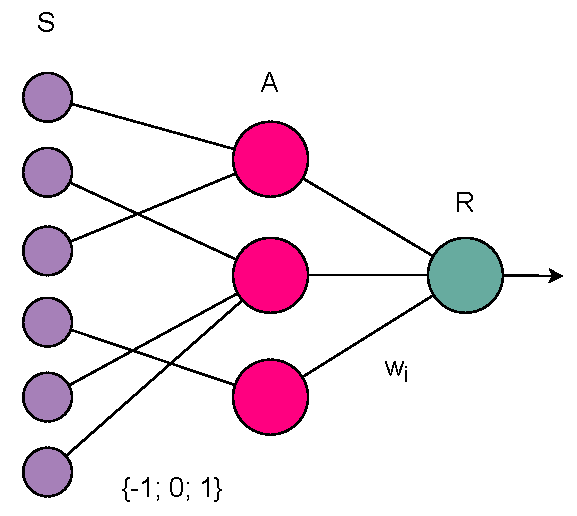
\includegraphics[scale=1]{img/perc.pdf}
	\caption{Схема перцептрона}
	\label{fig:Simple_perceptron}
\end{figure} 	

Кроме классического метода обучения перцептрона, Розенблат также ввел понятие об обучении без учителя, предложив следующий способ обучения: аль- фа-система подкрепления -- это система подкрепления, при которой веса всех активных связей, ведущих к элементу, изменяются на одинаковую величину r, а веса неактивных связей за это время не меняются.

Позже, с разработкой понятия многослойного перцептрона, альфа-система была модифицирована, и ее стали называть дельта-правилом. Модификацию было проведено с целью сделать функцию обучения дифференцируемой (например, сигмоидною), что в свою очередь требуется для применения метода градиентного спуска, благодаря которому возможно обучение более одного слоя.

В модели перцептрона используется один нейрон с линейной взвешенной сетевой и пороговой функциями активации. Входным сигналом для этого нейрона $x=(x_1,...,x_n)$ является вектор признаков в n-мерном пространстве признаков. Функция $f(x)$- это взвешенная сумма входных данных:
\begin{equation}
	f(x)=w_0 + \sum_{i=1}^{n}w_ix_i
\end{equation}

Обучение - это процесс, посредством которого свободные параметры нейронной сети адаптируются посредством непрерывного процесса стимуляции со стороны среды, в которую встроена сеть \cite{ettaouil2013architecture}. Тип обучения определяется способом, которым происходят изменения параметров. 

Алгоритм обучения перцептрона может быть реализован на электронном устройстве, и сеть становится в определенном смысле самоподстраивающейся. По этой причине процедуру подстройки весов обычно называют «обучением» и говорят, что сеть <<обучается>>. 

\subsubsection{Вывод}
В качестве нейронной сети была выбрана сеть Кохонена, так как заранее известно необходимое число кластеров. Немало важным фактором является устойчивость к шумам. Из-за того, что в выборке будут часто встречаться шумы, так как пользователи не всегда указывают полную информацию о себе и часто опускают некоторые данные, сеть Кохонена является наиболее подходящей для задачи персонализации пользователей социальных сетей для целевой рекламы.

\subsection{Выводы}
В данном разделе были проанализированы существующие программные решения, оказавшиеся в закрытом доступе, на основании чего было принято решение о разработке собственного метода персонализации пользователей социальных сетей.

Сравнительный анализ социальных сетей для решения задачи получения информации о пользователях выявил целесообразность использования API социальной сети ВКонтакте, так как оно является открытым и сама сеть не заблокирована на территории Российской Федерации.

Для решения задачи кластеризации была выбрана нейронная сеть Кохонена из-за ее устойчивости к шумам, высоком быстродействии, а также возможности обучения без начального указания общего числа кластеров.


\pagebreak